\subsection{Застосування нейронних мереж для отрмання маски людини}

Введемо поняття \textbf{маски людини (викладача)}.

Маскою людини \(F^{i}\) будемо називати бінарне прямокутне 
зображення \(M^{i}:P \rightarrow \left\{ 0,1 \right\}\), де тим
пікселям, в яких на відповідному кадрі \(F^{i}\) була помічена людина,
відповідає одиниця, а іншим відповідає нуль.

\subsection{Згорткові нейронні мережі (CNN)}

Для локалізації людини були використані так звані \textbf{згорткові нейронні мережі} 
(англ. \textit{convolutional neural networks, CNN}).
Це частина машинного навчання, яке називається глибоким навчанням, оскільки використовується 
більше двох нейронних шарів разом зі згортковими.

В таких меражах застосовується операція згортки(\textbf{Conv}) \textsf{}
та пулінгу (\textbf{Pooling}).

\begin{figure}[H]
    \centering
    \begin{subfigure}[c]{0.5\textwidth}
        \centering
        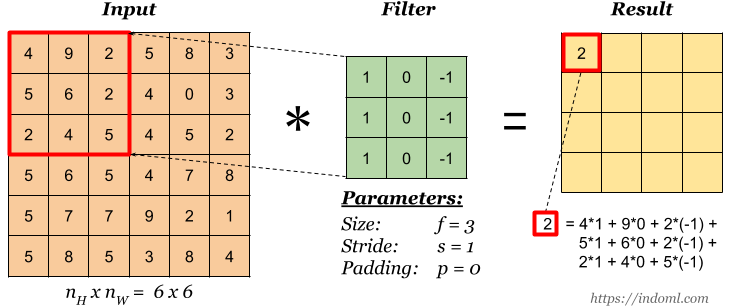
\includegraphics[width=\textwidth]{images/cnn_convolution_operation}
        \caption{Операція згортки
        \label{fig:cnn:operation}
        }
    \end{subfigure}
\end{figure}
\begin{figure}
    \centering
    \ContinuedFloat
    \begin{subfigure}[c]{0.5\textwidth}
        \centering
        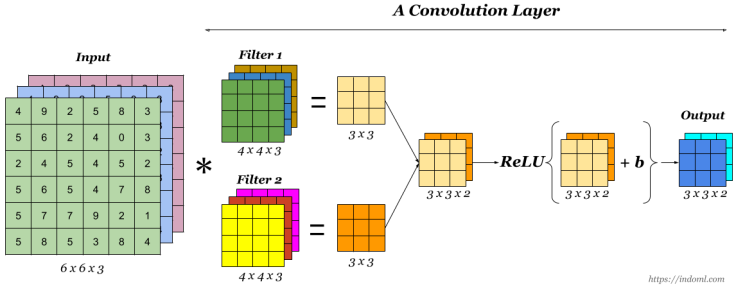
\includegraphics[width=\textwidth]{images/cnn_convolution_layer}
        \caption{Шар згортки
        \label{fig:cnn:layer}
        }
    \end{subfigure}
\end{figure}

Розглянемо архітектури нейронних мереж, що застосовувались у роботі
для детектингу людини. Всі нищеописані нейронні мережі були використані вже з
натренованими вагами у програмній бібліотеці PyTorch \cite{NEURIPS2019_9015}.
За мету було поставлено підібрати таку мережу, що здатна швидко оброблювати 
один знімок навіть на смартфоні. Тому головним критерієм є швидкість.

\textbf{YOLO}

YOLO (You-Only-Look-Once) - це сімейство нейронних мереж.

YOLOv1 вперше представили Joseph Redmon. 
Вона розв'язує задачу детекції об'єктів як задачу регресії
щодо просторового розділення знайдених областей об'єктів та їх
ймовірностей. Її зараз широко використовують для класифікації та знаходженні об'єктів
оскільки вона здатна оброблювати відео в реальному часі 30 кадрів в секунду 
на мобільних пристроях, ща є її найбільшою перевагою серед інших аналогів.

Опишемо коротко головні особливості YOLOv1, оскільки YOLOv5, яка застосовувалась 
в роботі є лише модифікацією:
\begin{enumerate}
    \item Спочтаку зображення розділяється решіткою $S \times S$.
          Якщо центр об'єкту потрапляє в комірку решітки, тоді ця комірка
          є кандидатом, для подальшого детектингу об'єкта.
    \item Кожна комірка решітки має передбачувати $B$ областей та рівнів
          довірів. Даний рівень довіри показує на скільки модель впевнена,
          що дана комірка містить об'єкт та на скільки точна область.
          Рівень довіри визначається $Pr(Object)*{IOU}_{pred}^{truth}$, 
          де $Pr(Object)$- ймовірність об'єкту, ${IOU}_{pred}^{truth}$ - величина
          перетину передбаченої області об'єкту до її справжньої.
          Відповідно якщо модель не знайшла об'єту цей рівень нульовий.
          Задача, щоб рівень довіри був якомога ближчим до ${IOU}_{pred}^{truth}$.
    \item Кожна область об'єкту складається з 5 чисел: рівень довіри,
          $x, y$ - координати центру об'єкту,  $w, h$ - його ширина та висота.
          Кожна комірка передбачає $C$ умовних йморівностей $Pr(Class_i|Object)$
\end{enumerate}

\begin{figure}[H]
    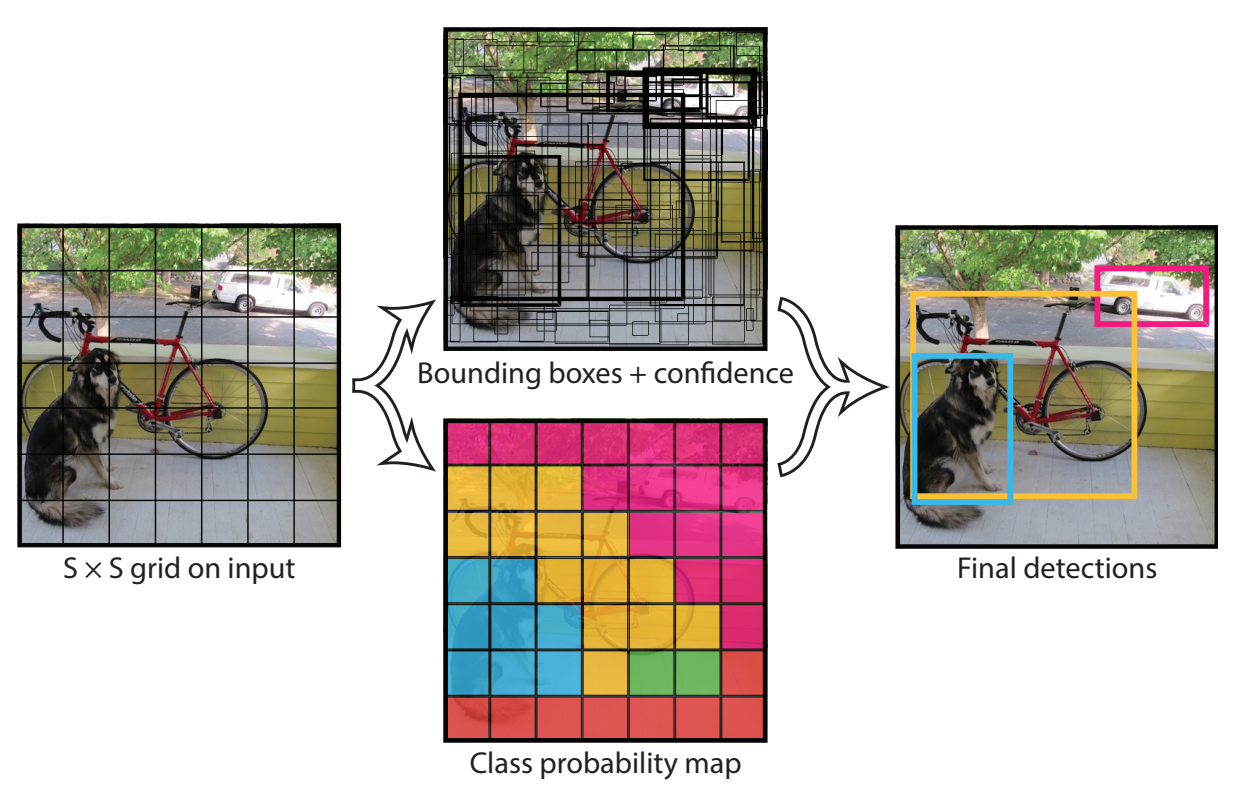
\includegraphics[width=0.5\linewidth]{images/cnn_yolo1}
    \centering
    \caption{Процес детектингу об'єктів мережею YOLO \cite{RedmonYolo}
    }
\end{figure}

Для тренування мережі використовують суму 4 штрафних функцій.

\begin{multline}
    \lambda_{coord}(
        \underbrace{ \sum_{i=0}^{S^2} \sum_{j=0}^{B} 
            \mathbb{1}_{ij}^{obj} [(x_i - \widehat{x_i})^2 + (y_i - \widehat{y_i})^2]
        }_\textrm{по координатам центру}\\
        +
        \underbrace{
        \sum_{i=0}^{S^2} \sum_{j=0}^{B} 
                \mathbb{1}_{ij}^{obj} [(\sqrt{w_i} - \sqrt{\widehat{w_i}})^2 + (\sqrt{h_i} - \sqrt{\widehat{h_i}})^2]
        }_\textrm{ширини та висоти об'єкту}
    )\\
    +  \underbrace{
        \sum_{i=0}^{S^2} \sum_{j=0}^{B} з
            \mathbb{1}_{ij}^{obj} (C_i - \widehat{C_i})^2
        +
        \lambda_{noobj} \sum_{i=0}^{S^2} \sum_{j=0}^{B} \mathbb{1}_{ij}^{noobj} (C_i - \widehat{C_i})^2 
        }_\textrm{точності класифікації}\\
    +  \underbrace{
        \sum_{i=0}^{S^2} \mathbb{1}_{i}^{nooobj}\sum_{c \in classes}(p_i(c) -  \widehat{p_i}(c))^2
        }_\textrm{ймовірності класів}
    \label{eq:cnn:yolo_loss}
\end{multline}
, де $\mathbb{1}_{i}^{obj}$ визначає чи знайшовся об'єкт в комірці $i$, а  
$\mathbb{1}_{ij}^{obj}$ чи в комірці $i$ в $j$-ій області знаходиться об'єкт.  

Загалом архітектура нейронної мережі YOLOv1 складається з 24 згорткових шарів та
2 повнозв'язних лінійних шарів.

\begin{figure}[H]
    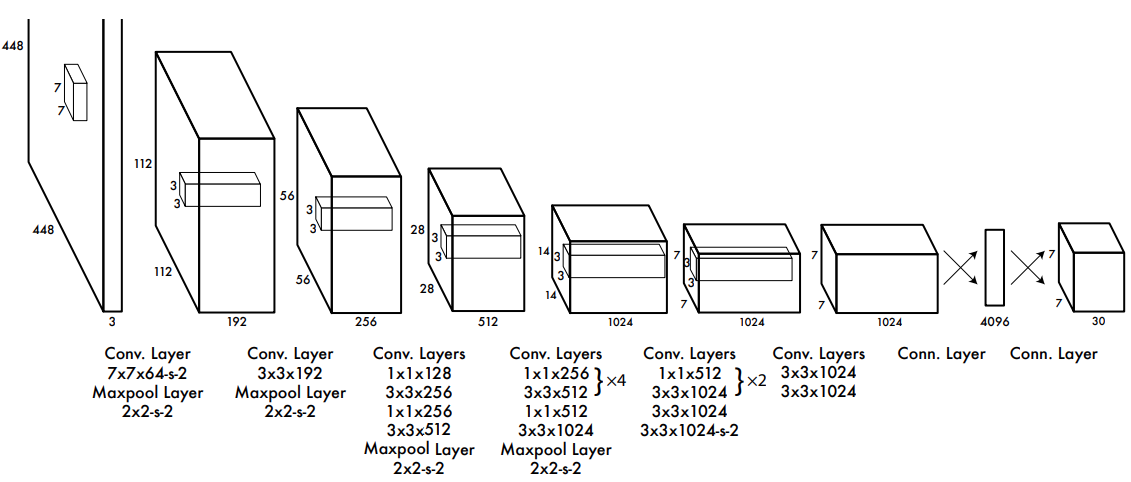
\includegraphics[width=0.8\linewidth]{images/cnn_yolo2}
    \centering
    \caption{Архітектура YOLOv1 \cite{RedmonYolo}
    }
\end{figure}

На момент написання була використана одна з мереж YOLOv5, яка була
розроблена Glenn Jocher вже на програмній бібліотеці PyTorch.

\begin{figure}[H]
    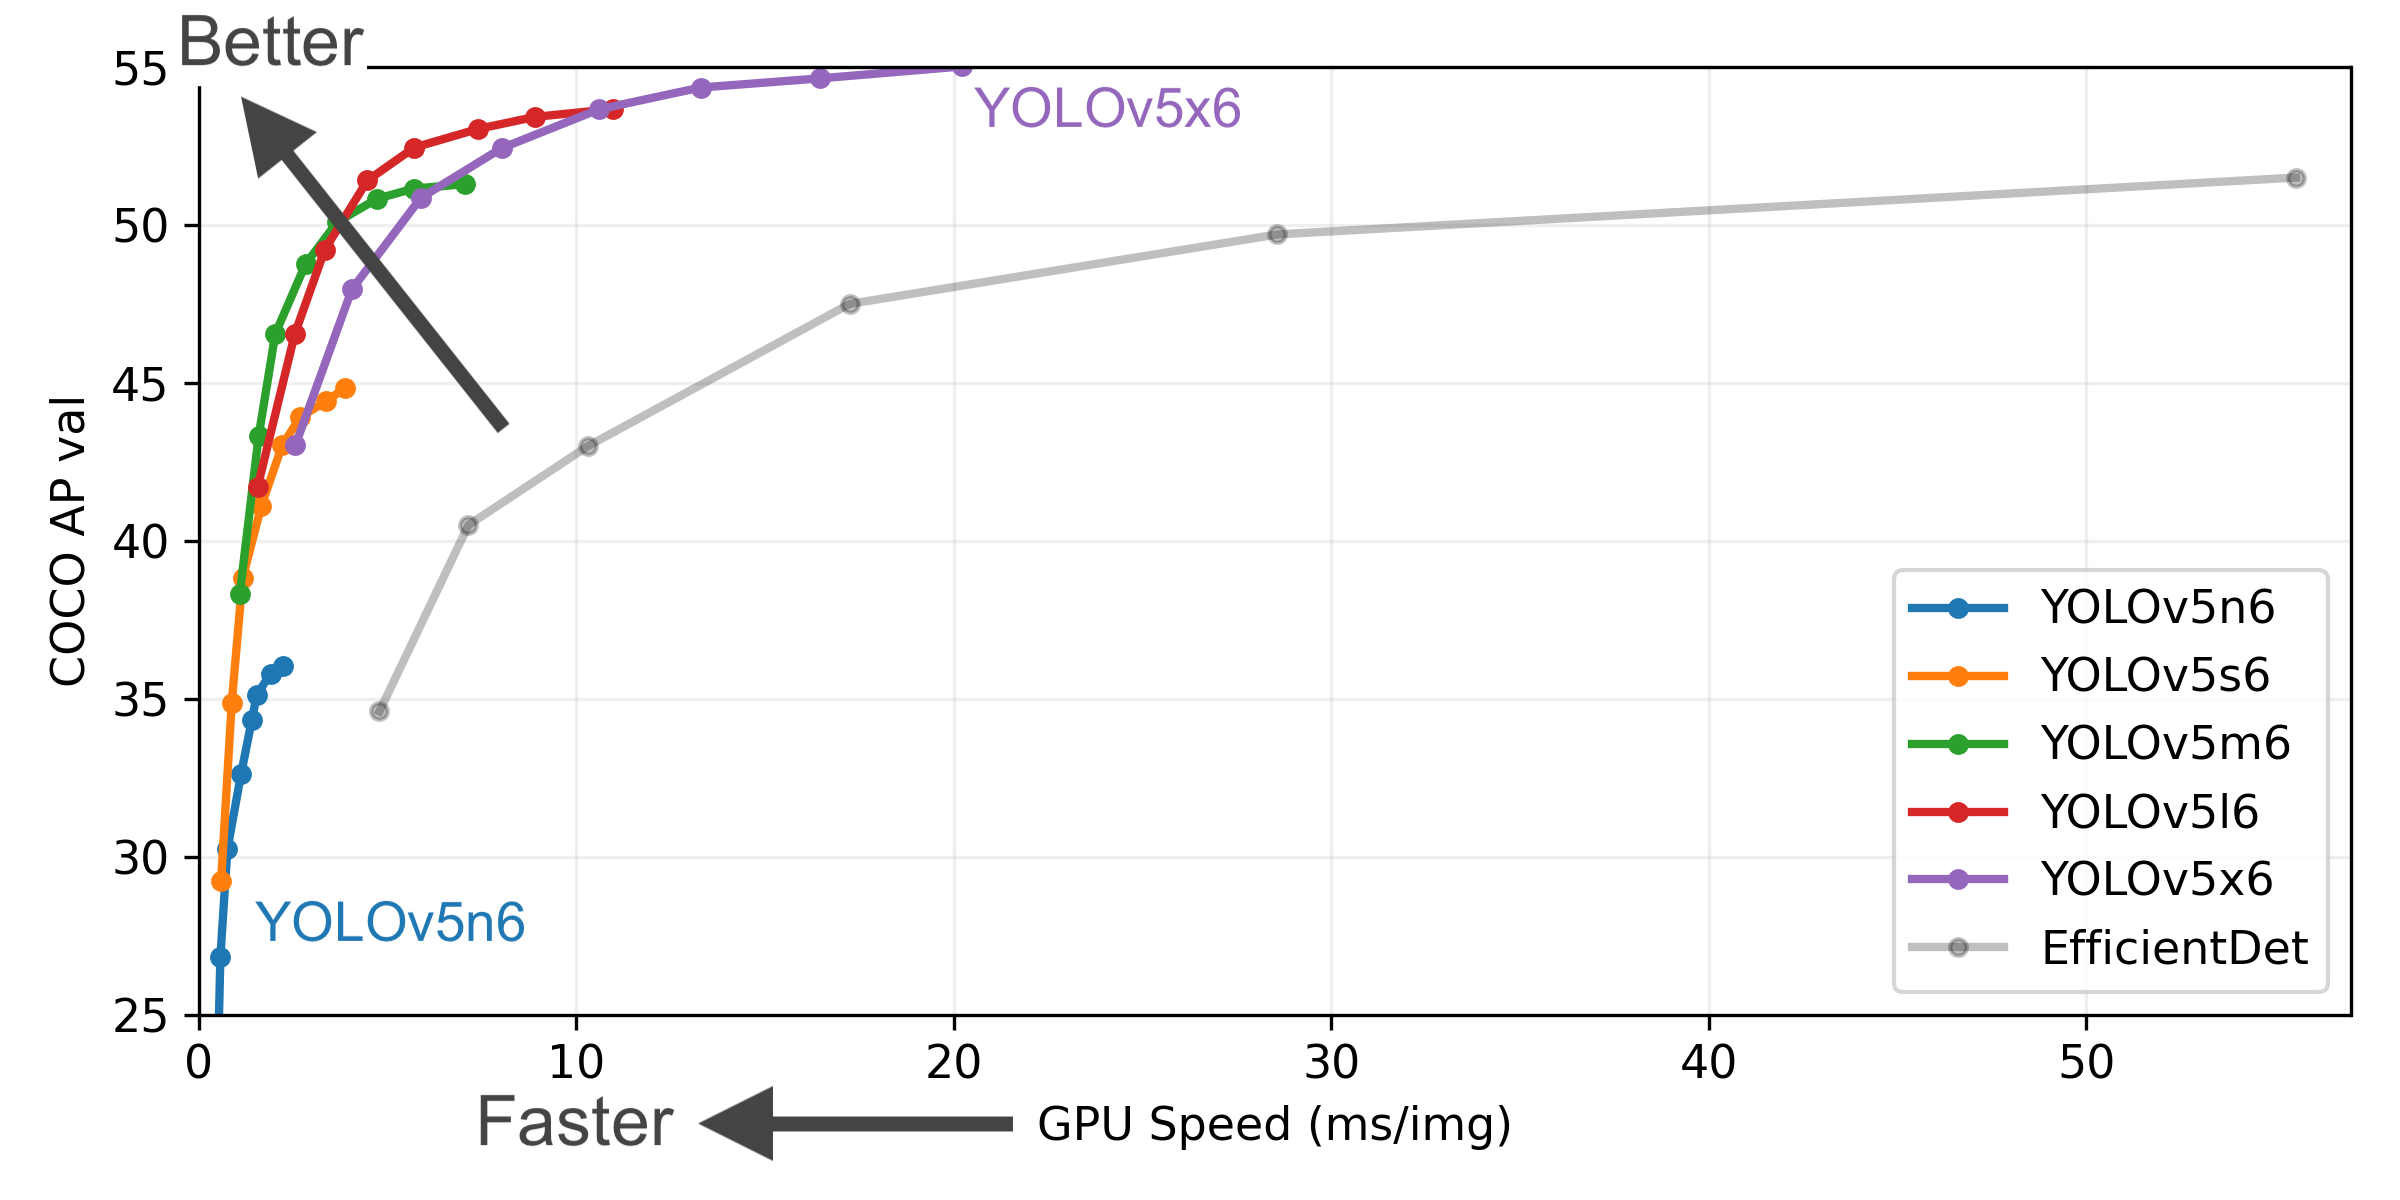
\includegraphics[width=0.5\linewidth]{images/cnn_yolo3}
    \centering
    \caption{Графік залежності точності  по датасеті COCO від швидкості обробки однієї 
    картинки різними мережами YOLOv5 н
    }
\end{figure}

\textbf{MobileNet}

MobileNet це також ще одне сімейство, що часто використовується у комп'ютерному зорі.
Вперше була представлена у 2017 році наковцями з Google.
З назви можна зрозуміти, що мета даної мережі як і вищеописаної це достатня продуктивність
на слабких обчислювальних системах.